\chapter{Influence of model parameters on metrics}
\label{chapter:Influence of model parameters on metrics}

In this chapter, we will examine how changes in the parameters affect the metrics discussed in sections \ref{sec:Fun Metric} and \ref{sec:Additional Metrics and Parameters}.

\section{The impact of vehicle density and composition on traffic flow}
\label{sec:The impact of vehicle density and composition on traffic flow}
In this section, the effect of vehicle $density$ on traffic flow is studied. The road curvature is kept constant and three different curvatures (400, 600, 900) are considered. The impact of the composition of vehicles on traffic flow is analyzed using two different $car\_share$ values (1 and 0.5). Finally, the effect of an increased number of motorcycles on traffic flow is analyzed.

\begin{figure}
     \centering
    \begin{subfigure}[b]{0.75\textwidth}
        \centering
        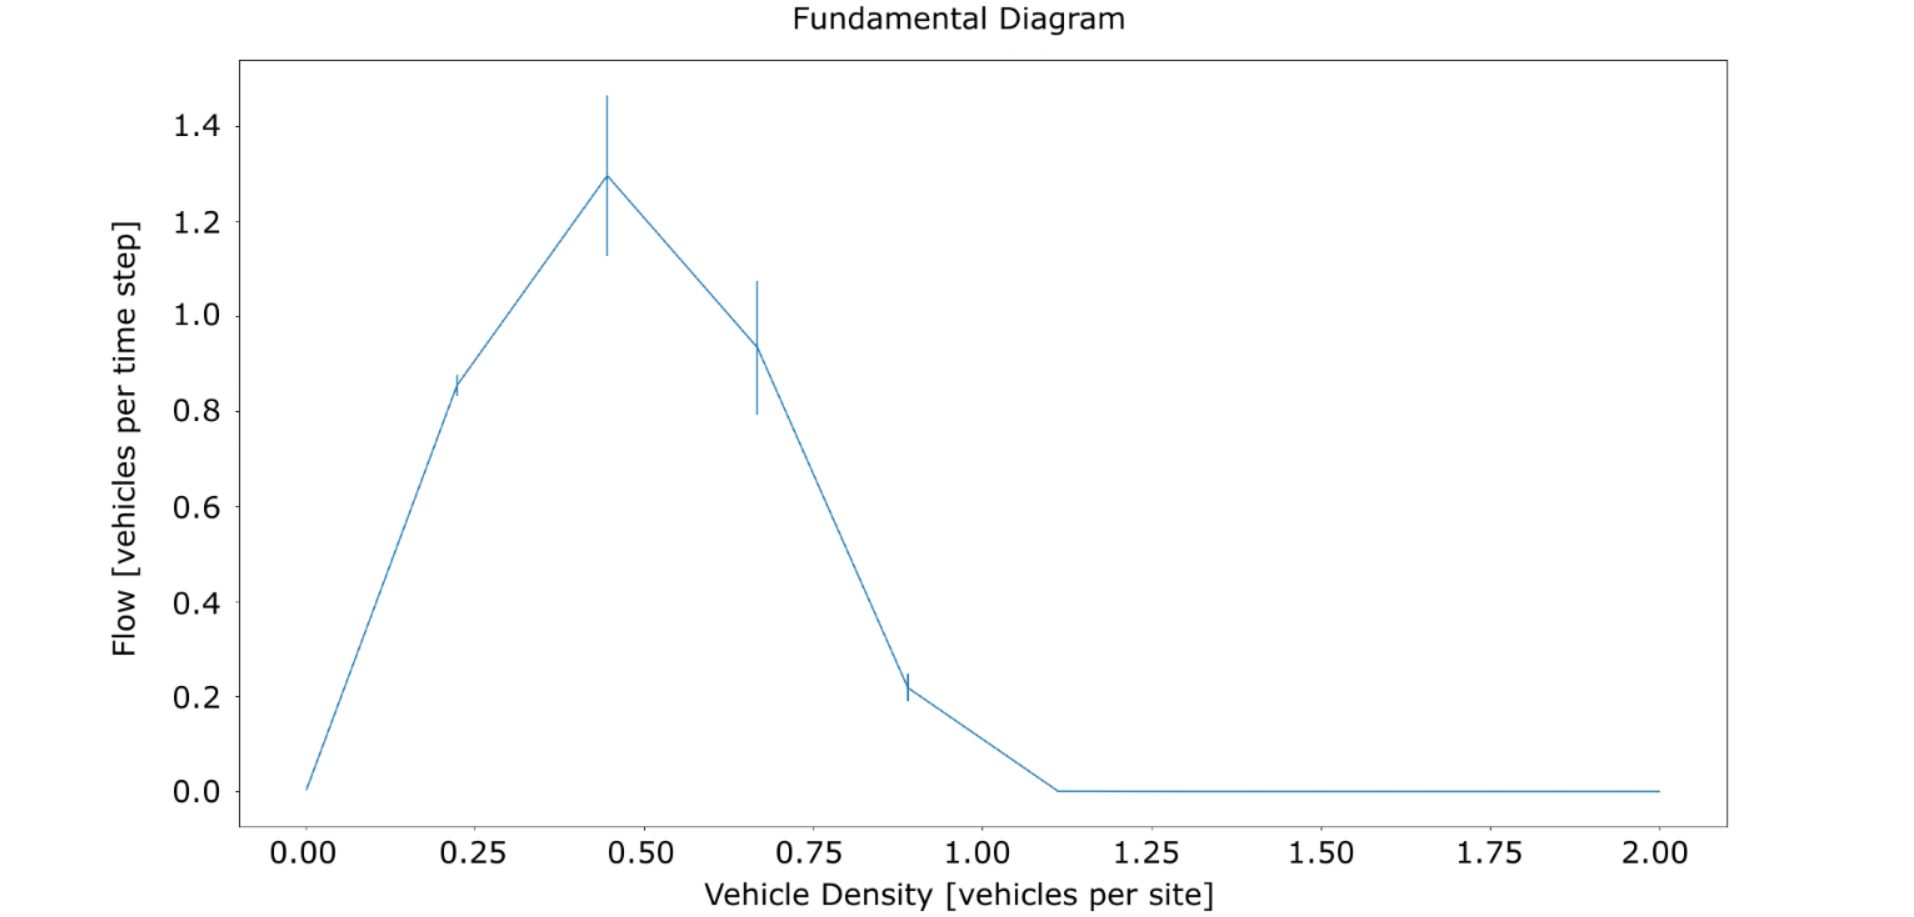
\includegraphics[width=\textwidth]{images/flow_density401_car_only.png}
        \caption{$density$ 400}
    \end{subfigure}
    \begin{subfigure}[b]{0.75\textwidth}
        \centering
        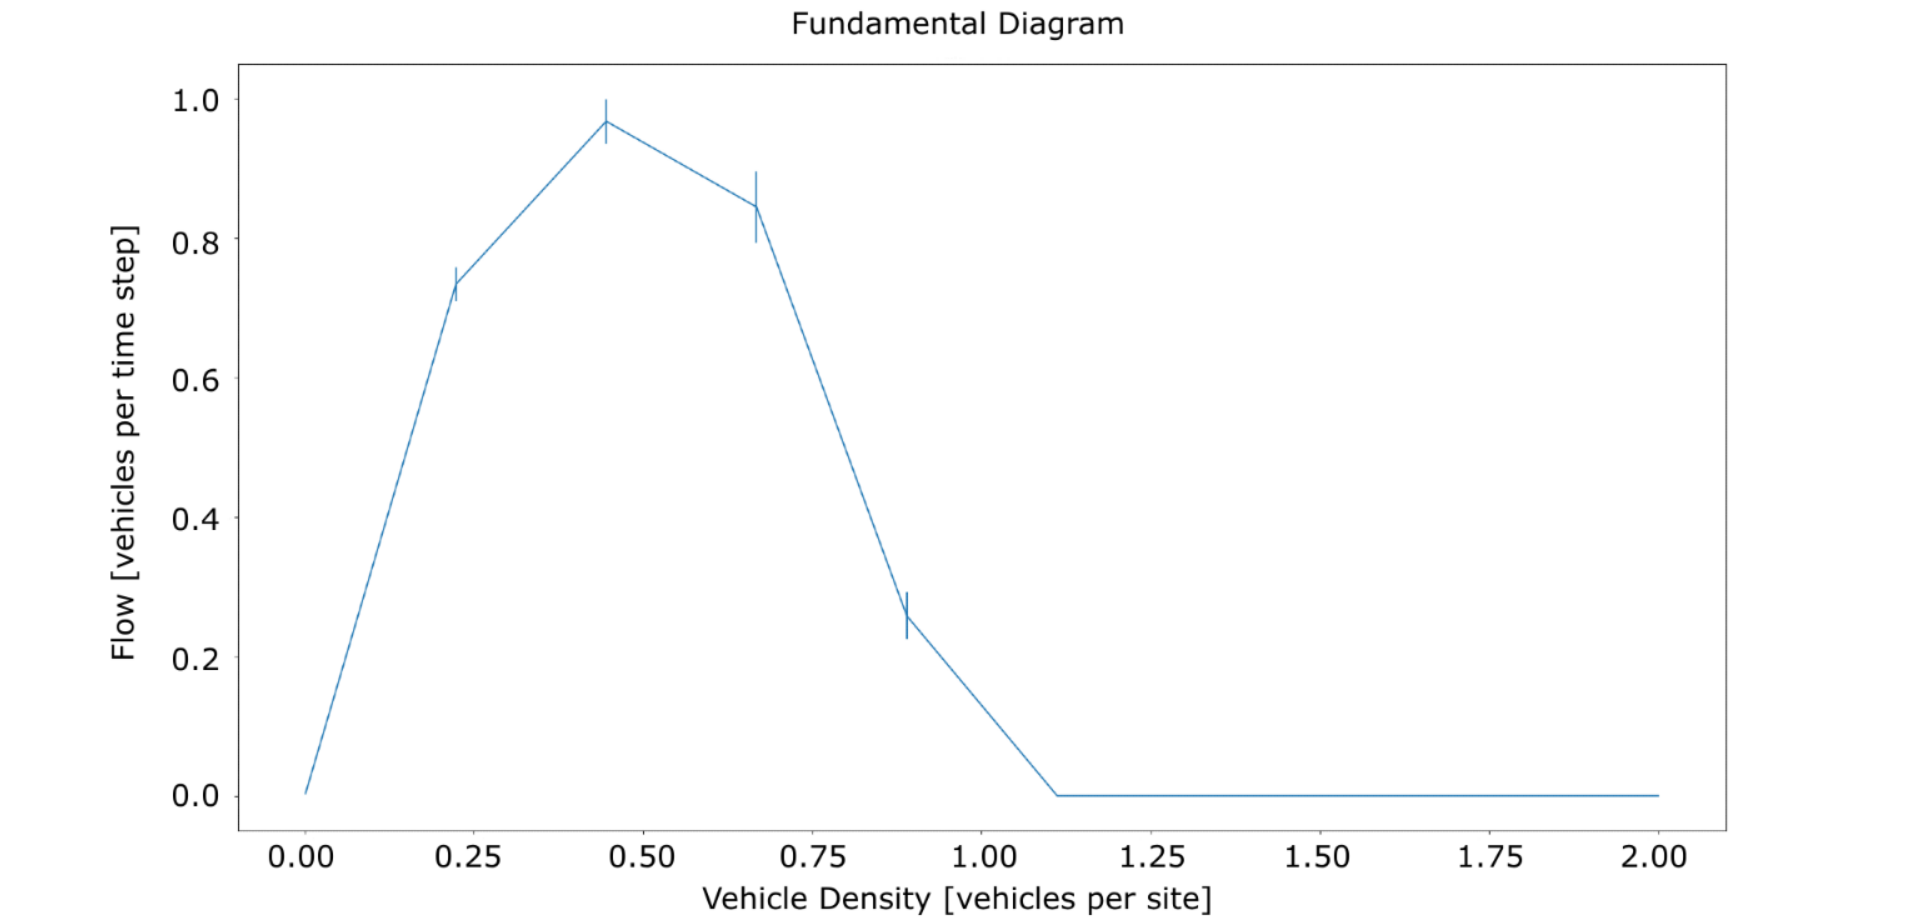
\includegraphics[width=\textwidth]{images/flow_density601_car_only.png}
        \caption{$density$ 600}
    \end{subfigure}
    \begin{subfigure}[b]{0.75\textwidth}
        \centering
        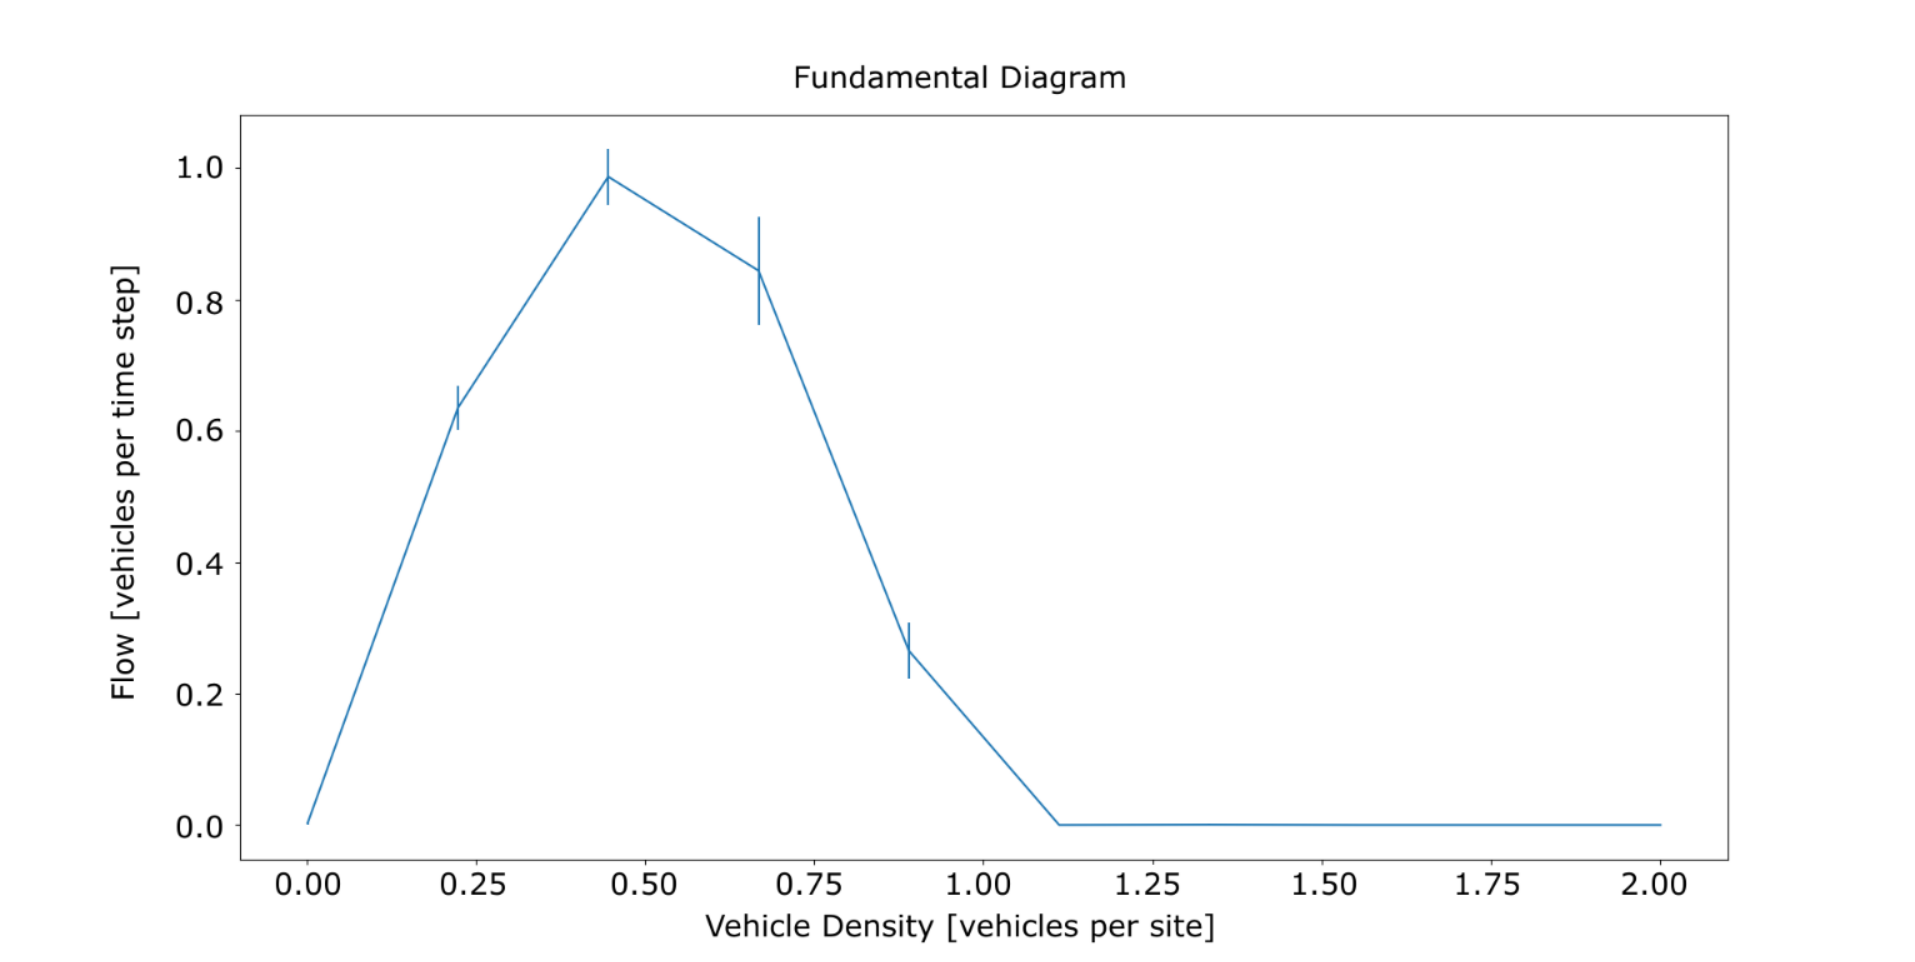
\includegraphics[width=\textwidth]{images/flow_density901_car_only.png}
        \caption{$density$ 900}
    \end{subfigure}
    \caption{This figure shows the flow-density diagram for a road of length 2000 tiles, with 200 time-steps and $car\_share$ 1, averaged over 10 loops for each value of the $density$ parameter. The diagram is shown for three different curvatures. The calculations for each diagram took approximately 1 hour to complete. The vertical line represents the standard deviation within a 95\% confidence interval of a normal distribution.}
    \label{fig:flow_density901_car_only}
\end{figure}

Figure \ref{fig:flow_density901_car_only} displays the flow-density diagrams for a street with a length of 2000 tiles and 200 time steps, where the traffic mainly consists of cars (with a negligible number of 5 motorcycles). The mean values are calculated from 10 loops for each $density$ value. The diagrams were generated for three different constant curvature values of the street. The figure shows that the peak on each diagram occurs at a $density$ of 0.4 vehicles for all curvature values. However, the height of the peak decreases from 1.3 vehicles per time-step passing through a section to about 1. This trend can be observed in all three diagrams. This is in line with the expectations as a higher curvature of the road forces the vehicles to drive at a slower speed. This observation is expected, as a higher curvature of the road forces the vehicles to drive at a slower speed. This in turn reduces the total flow of vehicles and reduces the maximum flow that the road can support. Interestingly, the height of the peak in the flow-density diagram does not increase from a curvature of 600 to 900. This unexpected result could be due to the imprecise calculation of the flow value that we discussed in Section \ref{sec:Additional Metrics and Parameters}. Specifically, the method for calculating the flow value involves counting all passing vehicles within 10 tiles at the beginning of the street at each time step, which could explain why the peak height does not decrease much with increasing curvature as the vehicle speed has less impact on the flow.
When compared to the flow-density diagram from K. Nagel and M. Schreckenberg (see figure \ref{fig:nasch_flow_density_diagram}), the results show a similar curve shape with a rapid increase in flow at higher densities. However, the peak $density$ occurs at 40\% on the two-lane road, more than twice the value of Nagel and Schreckenberg's single lane road, which could be attributed to the ability of vehicles to switch lanes and avoid congestion. The height of the maximum flow in the simulation can be explained by the fact that we are modeling a country road, where vehicles are limited by their speed, rather than a highway. Furthermore, the flow-density diagram in the simulation shows a steeper decrease compared to Figure \ref{fig:nasch_flow_density_diagram}. This could be due to the use of an asymmetric lane switching rule, where the right lane of the road experiences traffic jams at vehicle $density$ 1. This behavior is a result of the periodic boundary condition of the road, where the end of the road is connected to its beginning, causing the traffic to pile up on the right lane.\\


\begin{figure}
     \centering
    \begin{subfigure}[b]{1.0\textwidth}
        \centering
        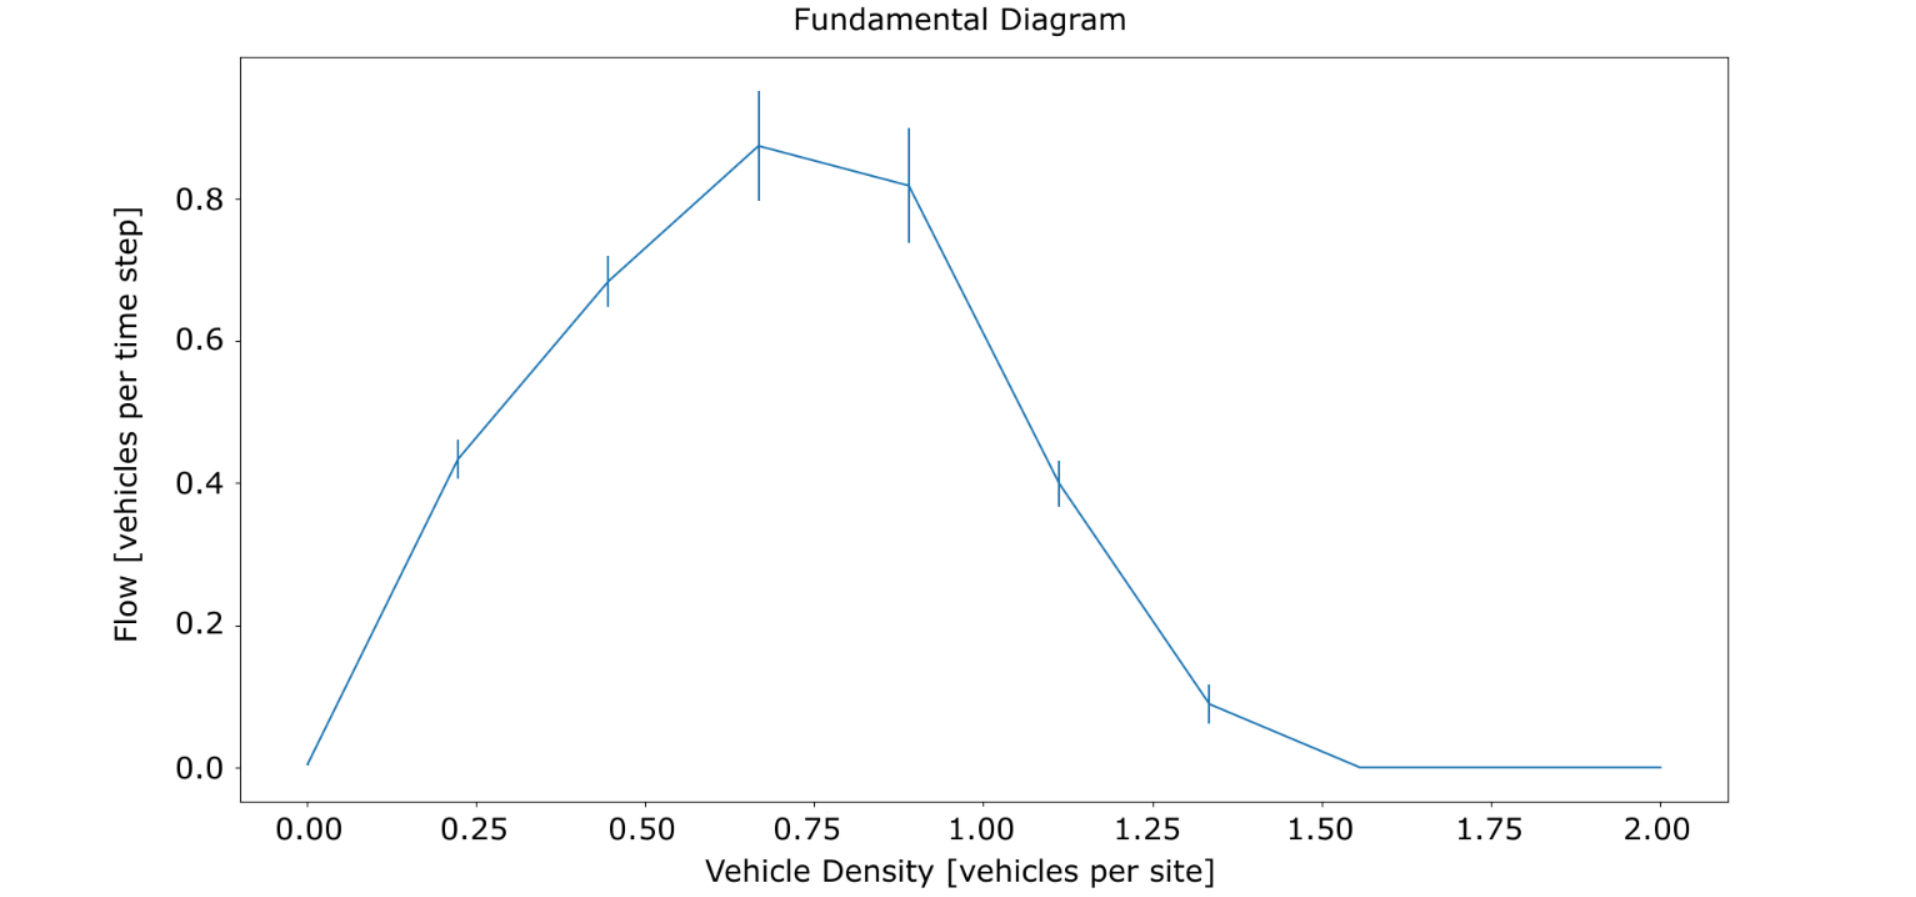
\includegraphics[width=\textwidth]{images/flow_density401_half_bike.png.png}
        \caption{Density 400}
    \end{subfigure}

    \begin{subfigure}[b]{1.0\textwidth}
        \centering
        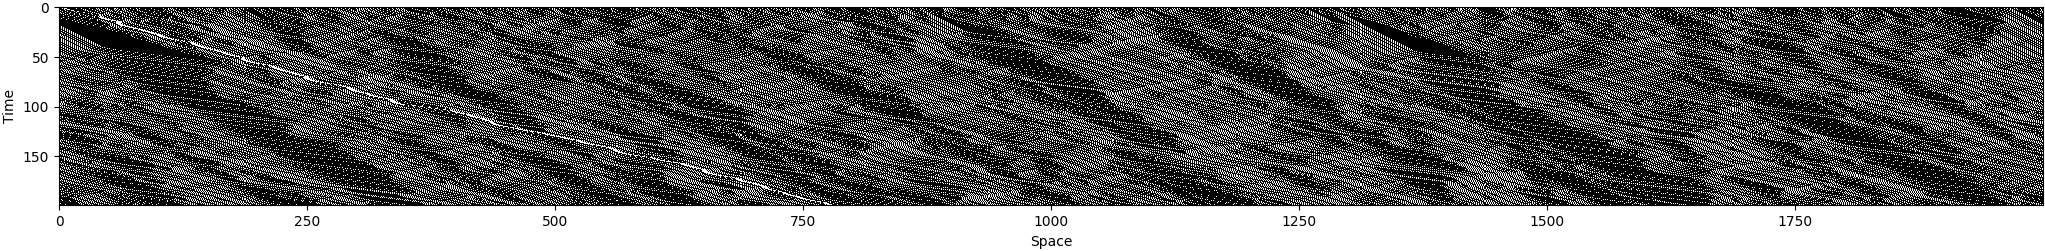
\includegraphics[width=\textwidth]{images/2D_401_half_bike_left.png}
        \caption{Density 400, left lane}
    \end{subfigure}

    \begin{subfigure}[b]{1.0\textwidth}
        \centering
        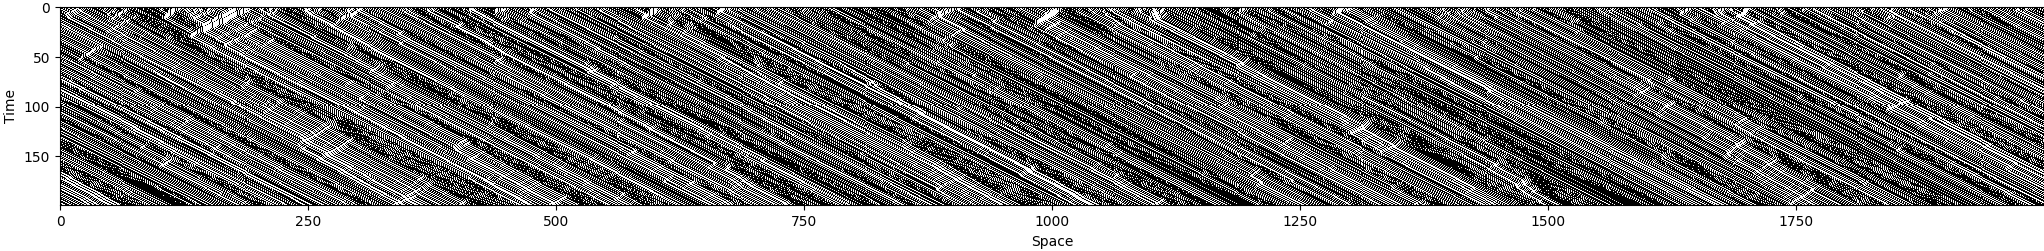
\includegraphics[width=\textwidth]{images/2D_401_half_bike_right.png}
        \caption{Density 400, right lane}
    \end{subfigure}
    \caption{This figure shows the flow-density diagram for a road of length 2000 tiles, with 200 time steps and $car\_share$ 0.5, averaged over 10 loops for street curvature 400. Calculation duration approximately 1h. The vertical line represents the standard deviation within a 95\% confidence interval of a normal distribution. The other two figures show 2D-pixel plots for the left and right lanes for a $density$ of 0.4, where white pixels represent the presence of a vehicle}
    \label{fig:flow_density401_half_bike}
\end{figure}

Figure \ref{fig:flow_density401_half_bike} displays the flow-density diagram for a simulation where half of the vehicles are bicycles, with the exception of 5 motorcyclists. The corresponding traffic movement and $density$ can be visualized in the two 2D-pixel plots that accompany the figure\footnote{In the 2D-pixel plot for the left lane, the presence of five motorcyclists is visible as a white line at the upper left corner of the plot.}. The x-axis of each plot represents the 2000-tile length of the street, while the y-axis represents time. Each line on the pixel plot corresponds to a time step in the simulation. 
The peak of the flow-density diagram occurs at a higher $density$ of 60\% when half of the vehicles are bicycles, compared to the case where all the vehicles are cars. This effect can be further observed in the 2D-pixel plot, where the bicyclists are seen moving to the right lane, which is indicated by a more cross line pattern on the right lane. At the same time, faster vehicles remain on the left lane, indicated by a laminar pattern on the left lane. This behavior allows the traffic to accommodate more vehicles before the flow collapses with increased $density$.\\

When the $car\_share$ is decreased to zero and only bicycles are present on the road, the flow-density diagram exhibits two local peaks, see figure \ref{fig:flow_density401_full_bike}. This effect can be attributed to the lane switching behavior of the bicyclists, who are modeled to stay on the right lane. However, as the $density$ of bicycles increases, the right lane becomes increasingly congested, leading to a reduction in flow and the emergence of the first local peak. The second peak arises as more and more bicyclists are forced to use the left lane, resulting in the utilization of both lanes and a subsequent increase in flow. \\

For the next analysis, the number\footnote{A higher number would lead eventually to a RecursionError.} of motorcyclists is increased from 5 to 200 and the $car\_share$ set to 0.9, which means that there would always be 200 motorcyclists on the road regardless of the $density$. Figure \ref{fig:flow_density401_more_bikers.png} shows the resulting flow-density diagram, which was generated by running the simulation ten times for each $density$. As expected, the flow-density diagram shows a shift in the peak to the right at vehicle $density$ of 0.7. Furthermore, the peak flow is lower at a vehicle density of 0.8 compared to a car only scenario, as shown in figure \ref{fig:flow_density901_car_only}. In addition, the shape of the flow density graph decreased more abruptly. It is suggested that this is because the platoon cannot use the road more efficiently because they are chained together compared to cars. 

\begin{figure}
	\centering
	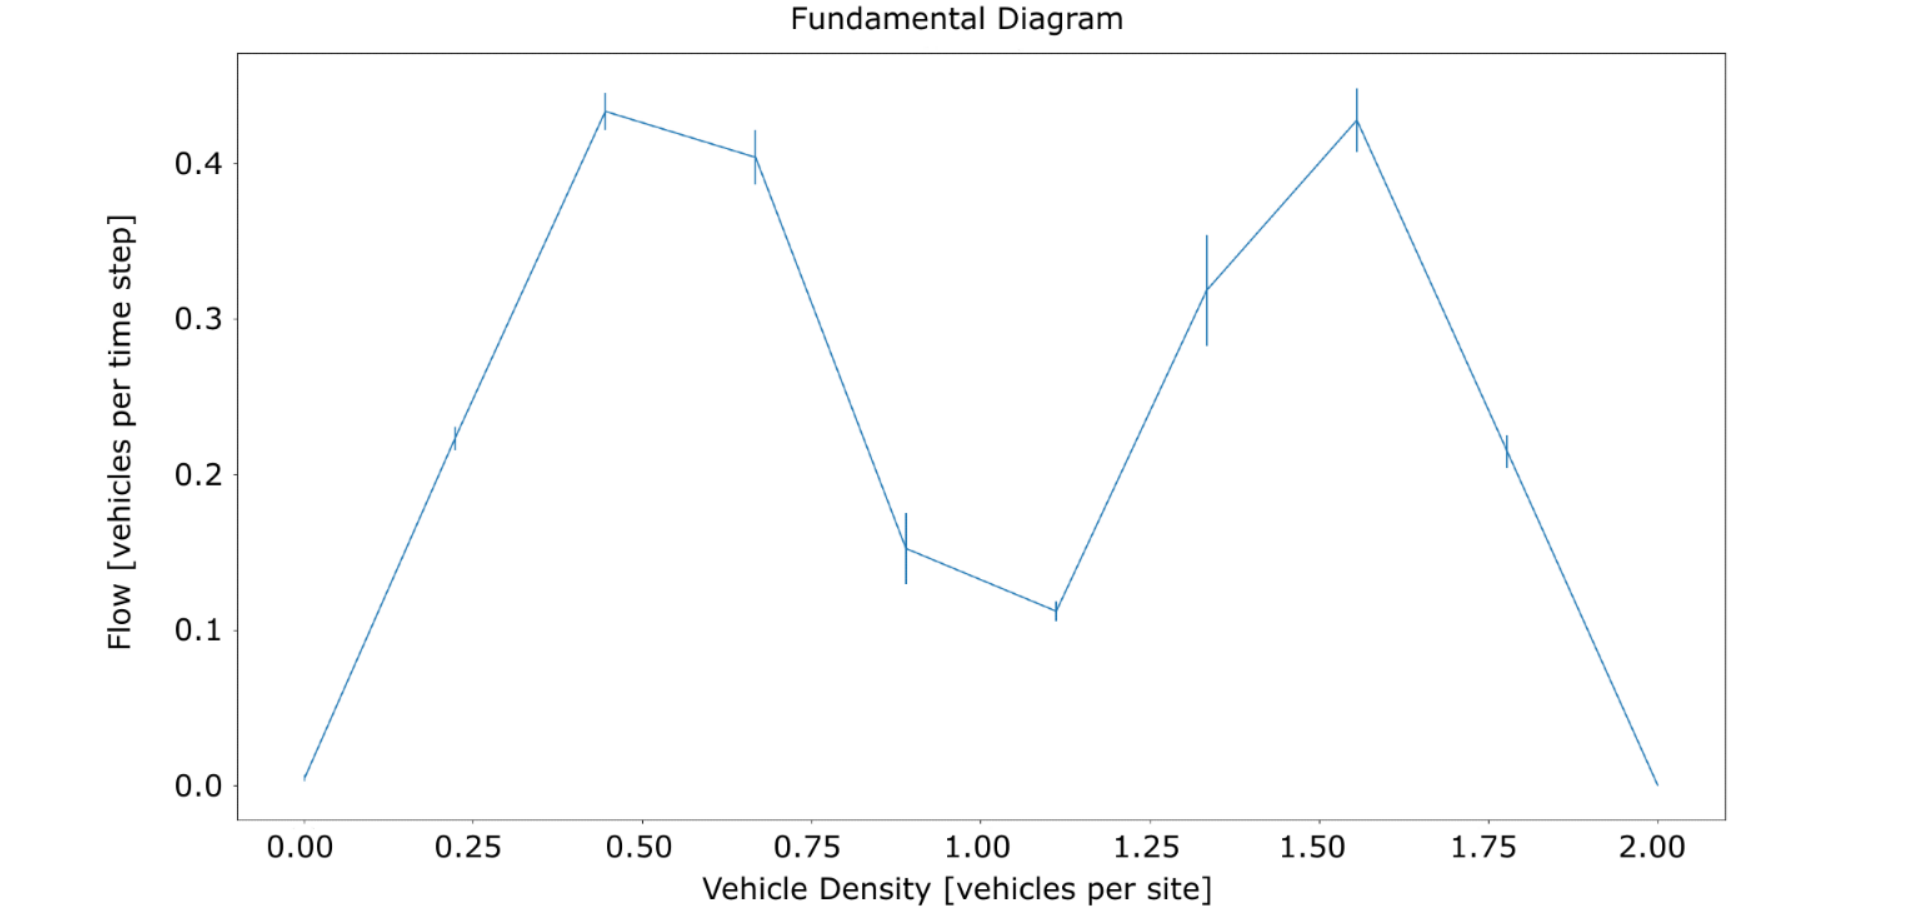
\includegraphics[width=1.0\linewidth]{images/flow_density401_full_bike.png}
	\caption{This figure shows the flow-density diagram for a road of length 2000 tiles, with 200 time steps and $car\_share$ 0.0, averaged over 10 loops for street curature 400. Calculation duration approximately 1h. The vertical line represents the standard deviation within a 95\% confidence interval of a normal distribution.}
	\label{fig:flow_density401_full_bike}
\end{figure}

\begin{figure}
    \centering
    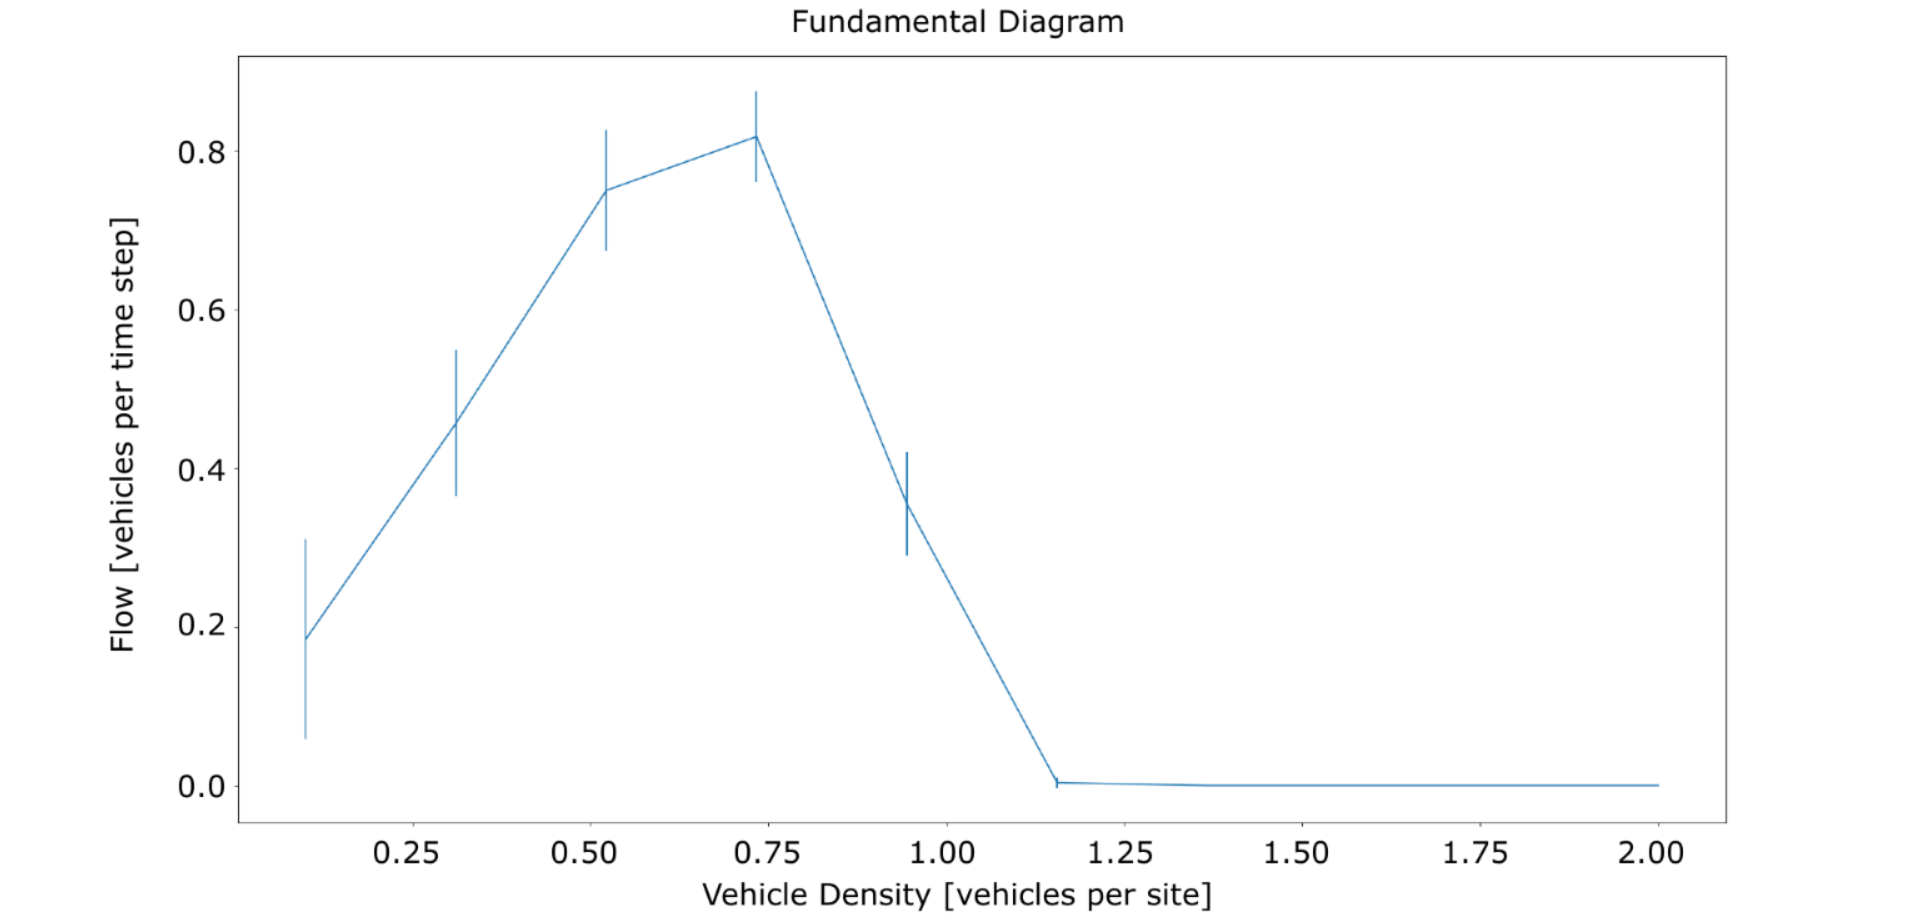
\includegraphics[width=1.0\linewidth]{images/flow_density401_more_bikers.png}
    \caption{The figure shows the flow-density diagram for a 2000-tile road with 200 time steps, 200 motorcyclists, and a $car\_share$ of 0.9. The diagram was generated by averaging the results of 10 simulation loops, with a street curvature of 400. Calculation duration approximately 1h. The vertical line represents the standard deviation within a 95\% confidence interval of a normal distribution.}
    \label{fig:flow_density401_more_bikers.png}
\end{figure}





